\chapter{Signal characterization}

Mathematics is full of complementary principles and symmetry.  Perhaps nowhere is this more evident than with \textit{inverse functions}: functions that ``un-do'' one another when put together.  A few examples of inverse functions are shown in the following table: \index{Inverse function} \index{Function, inverse}

% No blank lines allowed between lines of an \halign structure!
% I use comments (%) instead, so Tex doesn't choke.

$$\vbox{\offinterlineskip
\halign{\strut
\vrule \quad\hfil # \ \hfil & 
\vrule \quad\hfil # \ \hfil \vrule \cr
\noalign{\hrule}
%
% First row
$f(x)$ & $f^{-1}(x)$ \cr
%
\noalign{\hrule}
%
% Another row
Addition & Subtraction \cr
%
\noalign{\hrule}
%
% Another row
Multiplication & Division \cr
%
\noalign{\hrule}
%
% Another row
Power & Root \cr
%
\noalign{\hrule}
%
% Another row
Exponential & Logarithm \cr
%
\noalign{\hrule}
%
% Another row
Derivative & Integral \cr
%
\noalign{\hrule}
} % End of \halign 
}$$ % End of \vbox

Inverse functions are vital to master if one hopes to be able to manipulate algebraic (literal) expressions.  For example, to solve for time ($t$) in this exponential formula, you must know that the natural logarithm function directly ``un-does'' the exponential $e^x$.  This is the only way to ``unravel'' the equation and get $t$ isolated by itself on one side of the equals sign:

\begin{align*}
	V &= 12e^{-t}\\
\textit{Divide both sides by 12}\\
	\dfrac {V} {12} &= e^{-t}\\
	\textit{Take the natural logarithm of both sides}\\
	\ln \left(\dfrac {V}  {12}\right) &= \ln \left(e^{-t}\right)\\
\textit{The natural logarithm ``cancels out'' the exponential}\\
	\ln \left(\dfrac{V} {12}\right) &= -t\\
\textit{Multiply both sides by negative one}\\
	- \ln \left(\dfrac{V}{12}\right) &= t\\
\end{align*}




In industry there exist a great many practical problems where inverse functions play a similar role.  Just as inverse functions are useful for manipulating literal expressions in algebra, they are also useful in inferring measurements of things we cannot directly measure.  Many continuous industrial measurements are \textit{inferential} in nature, meaning that we actually measure some other variable in order to quantify the variable of interest.  More often than not, the relationship between the primary variable and the inferred variable is nonlinear, necessitating some form of mathematical processing to complete the inferential measurement. \index{Inferred variable}

Practical examples of inferential measurement include:

\begin{itemize}
\item Liquid flow measurement through restrictions in pipes
\item Liquid flow measurement in open channels (over weirs)
\item Liquid level measurement in non-cylindrical vessels
\item Temperature measurement by radiated energy
\item Chemical composition measurement
\end{itemize}

The following sections will describe the mathematics behind each of these measurement applications.






\filbreak
\section{Flow measurement from differential pressure}

Take for instance the problem of measuring fluid flow through a pipe.  To the layperson, this may seem to be a trivial problem.  However there is no practical way to \textit{directly} and continuously measure the flow rate of a fluid, especially when we cannot allow the fluid in question to become exposed to the atmosphere (e.g. when the liquid or gas in question is toxic, flammable, under high pressure, or any combination thereof).

One standard way to measure the flow rate of a fluid through a pipe is to intentionally place a restriction in the path of the fluid, and measure the pressure drop across that restriction.  The most common form of intentional restriction used for this purpose is a thin plate of metal with a hole precisely machined in the center, called an \textit{orifice plate}.  

\filbreak

A side view of the orifice plate assembly and pressure-measuring instrument looks like this: \index{Orifice plate}

$$\includegraphics{inverse_001.eps}$$

This approach should make intuitive sense: the faster the flow rate of the fluid, the greater the pressure difference developed across the orifice.  The actual physics of this process has to do with energy exchanging between potential and kinetic forms, but that is incidental to this discussion.  The mathematically interesting characteristic of this flow measurement technique is its nonlinearity.  Pressure does not rise linearly with flow rate; rather, it increases with the \textit{square} of the flow rate:

$$\includegraphics{inverse_002.eps}$$

To write this as a proportionality, we relate flow rate ($Q$) to pressure ($P$) as follows (the constant $k$ accounts for unit conversions and the geometries of the orifice plate and pipe):

$$P = k Q^2$$

\filbreak

This is a practical problem for us because our intent is to use pressure measurement ($P$) as an indirect (inferred) indication of flow rate ($Q$).  If the two variables are not \textit{directly} related to one another, we will not be able to regard one as being directly representative of the other.  To make this problem more clear to see, imagine a pressure gauge connected across the restriction, with the face of the gauge labeled in percent:  \index{Inferred variable}

$$\includegraphics{inverse_003.eps}$$

Consider a pressure gauge such as the one shown above, registering 20 percent on a linear scale at some amount of flow through the pipe.  What will happen if the flow rate through that pipe suddenly doubles?  An operator or technician looking at the gauge \textit{ought} to see a new reading of 40 percent, if indeed the gauge is supposed to indicate flow rate.  However, this will not happen.  Since the pressure dropped across the orifice in the pipe increases with the square of flow rate, a doubling of flow rate will actually cause the pressure gauge reading to \textit{quadruple!}  In other words, it will go from reading 20\% to reading 80\%, which is definitely not an accurate indication of the flow increase.

\filbreak

A couple of simple solutions exist for addressing this problem.  One is to re-label the pressure gauge with a ``square root'' scale.  Examine this photograph of a 3-15 PSI receiver gauge: \index{Square root scale} \index{Receiver gauge}

$$\includegraphics[width=4in]{inverse_022.eps}$$

Now, a doubling of fluid flow rate still results in a quadrupling of needle motion, but due to the nonlinear (inner) scale on this gauge this needle motion translates into a simple doubling of indicated flow, which is precisely what we need for this to function as an accurate flow indicator.

\filbreak

If the differential pressure instrument outputs a 4-20 mA analog electronic signal instead of a 3-15 PSI pneumatic signal, we may apply the same ``nonlinear scale'' treatment to any current meter and achieve the same result:

$$\includegraphics[width=4in]{inverse_026.eps}$$

Another simple solution is to use a \textit{nonlinear manometer}, with a curved viewing tube\footnote{This solution works best for measuring the flow rate of gases, not liquids, since the manometer obviously must use a liquid of its own to indicate pressure, and mixing or other interference between the process liquid and the manometer liquid could be problematic.}:  \index{Manometer, nonlinear}  \index{Nonlinear manometer} \index{Curved manometer}

$$\includegraphics{inverse_019.eps}$$

The scale positioned alongside the curved viewing tube will be linear, with equal spacings between division marks along its entire length.  The vertical height of the liquid column translates pressure into varying degrees of movement along the axis of the tube by the tube's curvature.  Literally, any inverse function desired may be ``encoded'' into this manometer by fashioning the viewing tube into the desired (custom) shape without any need to print a nonlinear scale.

Shown here is a photograph of an actual curved-tube manometer.  This particular specimen does not have a scale reading in units of flow, but it certainly could if it had the correct curve for a square-root characterization:

$$\includegraphics[width=4in]{inverse_018.eps}$$

\vskip 10pt

\filbreak

A more sophisticated solution to the ``square root problem'' is to use a computer to manipulate the signal coming from the differential pressure instrument so the characterized signal becomes a direct, linear representation of flow.  In other words, the computer \textit{square-roots} the pressure sensor's signal in order that the final signal becomes a direct representation of fluid flow rate: \index{Square root characterizer}

$$\includegraphics{inverse_005.eps}$$

Both solutions achieve their goal by mathematically ``un-doing'' the nonlinear (square) function intrinsic to the physics of the orifice plate with a complementary (inverse) function.  This intentional compounding of inverse functions is sometimes called \textit{linearization}, because it has the overall effect of making the output of the instrument system a direct proportion of the input: \index{Linearization}

$${Output} = k ({Input})$$




\filbreak
\section{Flow measurement in open channels}

Measuring the flow rate of liquid through an open channel is not unlike measuring the flow rate of a liquid through a closed pipe: one of the more common methods for doing so is to place a restriction in the path of the liquid flow and then measure the ``pressure'' dropped across that restriction.  The easiest way to do this is to install a low ``dam'' in the middle of the channel, then measure the height of the liquid upstream of the dam as a way to infer flow rate.  This dam is technically referred to as a \textit{weir}, and three styles of weir are commonly used: \index{Weir}

$$\includegraphics{inverse_006.eps}$$

Another type of open-channel restriction used to measure liquid flow is called a \textit{flume}.  An illustration of a \textit{Parshall flume} is shown here: \index{Flume} \index{Parshall flume}

$$\includegraphics{inverse_007.eps}$$

\textit{Weirs} and \textit{flumes} may be thought of being somewhat like ``orifice plates'' and ``venturi tubes,'' respectively, for open-channel liquid flow.  Like an orifice plate, a weir or a flume generates a differential pressure that varies with the flow rate through it.  However, this is where the similarities end.  Exposing the fluid stream to atmospheric pressure means the differential pressure caused by the flow rate manifests itself as a difference in liquid height at different points in the channel.  Thus, weirs and flumes allow the indirect measurement of liquid flow by sensing liquid height.  An interesting feature of weirs and flumes is that although they are nonlinear primary sensing elements, their nonlinearity is quite different from that of an orifice. \index{Weir} \index{Flume}

\filbreak

Note the following transfer functions for different weirs and flumes, relating the rate of liquid flow through the device ($Q$) to the level of liquid rise upstream of the device (called ``head'', or $H$):

\vskip 10pt

$$Q = 2.48 \left( \tan {\theta \over 2} \right) H^{5 \over 2} {\hskip 20pt V-notch weir}$$

\vskip 10pt

$$Q = 3.367 L H^{3 \over 2} {\hskip 20pt Cippoletti weir}$$

\vskip 10pt

$$Q = 0.992 H^{1.547} {\hskip 20pt 3-inch wide throat Parshall flume}$$

\vskip 10pt

$$Q = 3.07 H^{1.53} {\hskip 20pt 9-inch wide throat Parshall flume}$$

\vskip 10pt

\noindent
Where,

$Q$ = Volumetric flow rate (cubic feet per second -- CFS)

$L$ = Width of notch crest or throat width (feet)

$\theta$ = V-notch angle (degrees)

$H$ = Head (feet)

\vskip 10pt

It is important to note these functions provide answers for flow rate ($Q$) with head ($H$) being the independent variable.  In other words, they will tell us how much liquid is flowing given a certain head.  In the course of calibrating the head-measuring instruments that infer flow rate, however, it is important to know the inverse transfer function: how much head there will be for any given value of flow.  Here, algebraic manipulation becomes important to the technician.  For example, here is the solution for $H$ in the function for a Cippoletti weir: \index{Cippoletti weir}

$$Q = 3.367 L H^{3 \over 2}$$

$$\textit{Dividing both sides of the equation by 3.367 and }L {:}$$

$${Q \over 3.367 L} =  H^{3 \over 2}$$

$$\textit{Taking the } {3 \over 2} { root of both sides:}$$

$$\root {3 / 2} \of {Q \over 3.367 L} =  H$$

\filbreak

This in itself may be problematic, as some hand calculators do not have an $\root x \of y$ function.  In cases such as this, it is helpful to remember that a root is nothing more than an inverse power.  Therefore, we could re-write the final form of the equation using a $2 \over 3$ power instead of a $3 \over 2$ root: \index{Powers and roots} \index{Roots and powers}

$$\left({Q \over 3.367 L}\right)^{2 \over 3} =  H$$






\filbreak
\section{Material volume measurement}

\label{Storage tank characterization}

A variety of technologies exist to measure the quantity of stored material in a vessel.  For liquid applications, hydrostatic pressure, radar, ultrasonic, and tape-and-float are just a few of the more common technologies:

$$\includegraphics{inverse_008.eps}$$

These measuring technologies share a common trait: they infer the quantity of material stored in the vessel by measuring \textit{height}.  If the vessel in question has a constant cross-sectional area throughout its working height (e.g. a vertical cylinder), then material height will directly correspond to stored material volume.  However, if the vessel in question does not have a constant cross-sectional area throughout its height, the relationship between material height and material volume will not be linear.

\filbreak

For example, there is a world of difference between the height/volume functions for a vertical cylinder versus a horizontal cylinder:

$$\includegraphics{inverse_016.eps}$$

The volume function for a vertical cylinder is a simple matter of geometry -- height ($h$) multiplied by the cylinder's cross-sectional area ($\pi r^2$):

$$V = \pi r^2 h$$

Calculating the volume of material stored inside a horizontal cylinder as a function of material height ($h$) is a far more complicated matter, because the cross-sectional area is not constant.  The solution to this problem is an exercise in integral calculus, the final result being this unwieldy function:

%Calculating the volume of a horizontal cylinder as a function of material height ($h$) is a far more complicated matter, because the cross-sectional area is also a function of height.  For this, we need to apply calculus.

%First, we begin with the mathematical definition of a circle, then graphically represent a partial area of that circle as a series of very thin rectangles:

%$$\includegraphics{inverse_015.eps}$$

%In this sketch, I show the circle ``filling'' from left to right rather than from bottom to top.  I have done this strictly out of mathematical convention, where the $x$ (horizontal) axis is the independent variable.  No matter how the circle gets filled, the relationship of area ($A$) to fill distance ($h$) will be the same.

%If $x^2 + y^2 = r^2$ (the mathematical definition of a circle), then the area of each rectangular ``slice'' comprising the accumulated area between $-r$ and $h-r$ is equal to $2y \> dx$.  In other words, the total accumulated area between $-r$ and $h-r$ is:

%$$A = \int_{-r}^{h-r} 2y \> dx$$

%Now, writing $y$ in terms of $r$ and $x$ ($y = \sqrt{r^2 - x^2}$) and moving the constant ``2'' outside the integrand:

%$$A = 2 \int_{-r}^{h-r} \sqrt{r^2 - x^2} \> dx$$

%Consulting a table of integrals, we find this solution for the general form:

%$$\int \sqrt{a^2 - u^2} \> du = {u \over 2} \sqrt{a^2 - u^2} + {a^2 \over 2} \sin^{-1}\left({u \over a}\right) + C$$

%\filbreak

%Applying this solution to our particular integral . . .

%$$A = 2 \left[ {x \over 2} \sqrt{r^2 - x^2} + {r^2 \over 2} \sin^{-1}\left({x \over r}\right) \right]_{-r}^{h-r}$$

%$$A = 2 \left[ \left( {(h-r) \over 2} \sqrt{r^2 - (h-r)^2} + {r^2 \over 2} \sin^{-1}{(h-r) \over r} \right) - \left( {-r \over 2} \sqrt{r^2 - (-r)^2} + {r^2 \over 2} \sin^{-1}{-r \over r} \right)\right]$$

%$$A = 2 \left[ \left( {(h-r) \over 2} \sqrt{r^2 - (h^2 -2hr + r^2)} + {r^2 \over 2} \sin^{-1}{(h-r) \over r} \right) - \left( {-r \over 2} \sqrt{0} + {r^2 \over 2} {-\pi \over 2} \right)\right]$$

%$$A = 2 \left[ \left( {(h-r) \over 2} \sqrt{2hr - h^2} + {r^2 \over 2} \sin^{-1}{(h-r) \over r} \right) - \left( {-\pi r^2 \over 4} \right)\right]$$

%$$A = \left[ (h-r) \sqrt{2hr - h^2} + r^2 \sin^{-1}{(h-r) \over r} + {\pi r^2 \over 2} \right]$$

%Knowing that the stored material volume in the horizontal tank will be this area multiplied by the constant length ($L$) of the tank, our formula for volume is as follows:

$$V = L \left[ (h-r) \sqrt{2hr - h^2} + r^2 \sin^{-1}{(h-r) \over r} + {\pi r^2 \over 2} \right]$$

Any instrumentation system inferring stored material volume by measurement of material height in a horizontal cylinder must somehow apply this formula on a continuous basis.  This is a prime example of how digital computer technology is essential to certain continuous measurement applications!

\vskip 10pt

\filbreak

Spherical vessels, such as those used to store liquefied natural gas (LNG) and butane, present a similar challenge: the material height/volume function is more complicated than for a vertical cylinder because the cross-sectional area of a spherical vessel changes with height.  Once again an exercise in integral calculus is necessary to derive a formula for calculating the stored volume of material inside a sphere based on material height:

$$\includegraphics{inverse_028.eps}$$

Whereas the material volume function for a vertical cylinder is a simple linear formula ($V = \pi r^2 h$), the material volume formula for a sphere is a bit more complicated although not as complicated as it is for a horizontal cylinder:

% ADD: If we were to graph the function relating level ($h$) to stored volume ($V$) within a hollow sphere, we would see something like this:
% $$\includegraphics{inverse_009.eps}$$

%Calculus provides a way for us to derive an equation solving for stored volume ($V$) with height ($h$) as the independent variable.  We begin in a similar manner to the last problem with the mathematical definition of a circle, except now we consider the filling of a sphere with a series of thin, circular disks:

%$$\includegraphics{inverse_017.eps}$$

%If $x^2 + y^2 = r^2$ (the mathematical definition of a circle), then the volume of each circular disk comprising the accumulated volume between $-r$ and $h-r$ is equal to $\pi y^2 \> dx$.  In other words, the total accumulated area between $-r$ and $h-r$ is:

%$$V = \int_{-r}^{h-r} \pi y^2 \> dx$$

%Now, writing $y$ in terms of $r$ and $x$ ($y = \sqrt{r^2 - x^2}$) and moving the constant $\pi$ outside the integrand:

%$$V = \pi \int_{-r}^{h-r} \left(\sqrt{r^2 - x^2}\right)^2 \> dx$$

%Immediately we see how the square and the square-root cancel one another, leaving us with a fairly simple integrand:

%$$V = \pi \int_{-r}^{h-r} r^2 - x^2 \> dx$$

%We may write this as the difference of two integrals:

%$$V = \left( \pi \int_{-r}^{h-r} r^2 \> dx \right) - \left( \pi \int_{-r}^{h-r} x^2 \> dx \right)$$

%\filbreak

%Since $r$ is a constant, the left-hand integral is simply $\pi r^2x$.  The right-hand integral is solvable by the power rule:

%$$V = \pi r^2 \left[ x \right]_{-r}^{h-r} - \left[ \pi {x^3 \over 3} \right]_{-r}^{h-r}$$

%$$V = \pi r^2 \left[(h-r) -(-r) \right] - \left[ \pi {(h-r)^3 \over 3} - \pi {(-r)^3 \over 3} \right]$$

%$$V = \pi r^2 \left[ h - r + r \right] - {\pi \over 3} \left[ (h-r)^3 - (-r)^3  \right]$$

%$$V = \pi hr^2 - {\pi \over 3} \left[ (h^3 - 2h^2r +hr^2 -h^2r +2hr^2 -r^3) + r^3  \right]$$

%$$V = \pi hr^2 - {\pi \over 3} \left[ h^3 - 3h^2r +3hr^2 \right]$$

%$$V = \pi hr^2 - {\pi h^3 \over 3} + \pi h^2r - \pi hr^2 $$

%$$V = - {\pi h^3 \over 3} + \pi h^2r $$

%$$V = \pi h^2r -  {\pi h^3 \over 3}$$

$$V = \pi h^2 \left(r - {h \over 3}\right)$$

This function will ``un-do'' the inherent height/volume nonlinearity of a spherical vessel, allowing a height measurement to translate directly into a volume measurement.  A ``characterizing'' function such as this is typically executed in a digital computer connected to the level sensor, or sometimes in a computer chip within the sensor device itself.

\filbreak

An interesting alternative to a formal equation for linearizing the level measurement signal is something called a \textit{multi-segment characterizer} function, typically implemented as a function block inside a digital loop controller or distributed control system (DCS).  This is an example of what mathematicians call a \textit{piecewise function}: a function made up of line segments.  Multi-segment characterizer functions may be programmed to emulate virtually any continuous function, with reasonable accuracy: \index{Piecewise function} \index{Function, piecewise} \index{Multi-segment characterizer}

$$\includegraphics{inverse_010.eps}$$

The computer correlates the input signal (height measurement, $h$) to a point on this piecewise function, linearly interpolating between the nearest pair of programmed coordinate points.  The number of points available for multi-point characterizers varies between ten and one hundred\footnote{There is no theoretical limit to the number of points in a digital computer's characterizer function given sufficient processing power and memory.  There is, however, a limit to the patience of the human programmer who must encode all the necessary $x,y$ data points defining this function.  Most of the piecewise characterizing functions I have seen available in digital instrumentation systems provide 10 to 20 ($x,y$) coordinate points to define the function.  Fewer than 10 coordinate points risks excessive interpolation errors, and more than 20 would just be tedious to configure.} depending on the desired accuracy and the available computing power.

\filbreak

Although true fans of math might blanch at the idea of approximating an inverse function for level measurement using a piecewise approach rather than simply implementing the correct continuous function, the multi-point characterizer technique does have certain practical advantages.  For one, it is readily adaptable to any shape of vessel, no matter how strange.  Take for instance this vessel, made of separate cylindrical sections welded together:

$$\includegraphics{inverse_011.eps}$$

Here, the vessel's very own height/volume function is fundamentally piecewise, and so \textit{nothing but} a piecewise characterizing function could possibly linearize the level measurement into a volume measurement!

Consider also the case of a spherical vessel with odd-shaped objects welded to the vessel walls, and/or inserted into the vessel's interior:

$$\includegraphics{inverse_012.eps}$$

The volumetric space occupied by these structures will introduce all kinds of discontinuities into the transfer function, and so once again we have a case where a continuous characterizing function cannot properly linearize the level signal into a volume measurement.  Here, \textit{only} a piecewise function will suffice.

\filbreak

To best generate the coordinate points for a proper multi-point characterizer function, one must collect data on the storage vessel in the form of a \textit{strapping table}.  This entails emptying the vessel completely, then filling it with measured quantities of material, one sample at a time, and taking level readings.  The result of this exercise is a data table correlating known volumes of material inside the vessel with measured heights of that material:  \index{Strapping table}  \index{Table, strapping}

% No blank lines allowed between lines of an \halign structure!
% I use comments (%) instead, so Tex doesn't choke.

$$\vbox{\offinterlineskip
\halign{\strut
\vrule \quad\hfil # \ \hfil & 
\vrule \quad\hfil # \ \hfil \vrule \cr
\noalign{\hrule}
%
% First row
\textbf{Introduced material volume} & \textbf{Measured material level} \cr
%
\noalign{\hrule}
%
% Another row
150 gallons & 2.46 feet \cr
%
\noalign{\hrule}
%
% Another row
300 gallons & 4.72 feet \cr
%
\noalign{\hrule}
%
% Another row
450 gallons & 5.8 feet \cr
%
\noalign{\hrule}
%
% Another row
600 gallons & (etc., etc.) \cr
%
\noalign{\hrule}
%
% Another row
750 gallons & (etc., etc.) \cr
%
\noalign{\hrule}
} % End of \halign 
}$$ % End of \vbox

Each of these paired numbers would constitute the coordinates to be programmed into the characterizer function computer by the instrument technician or engineer:

$$\includegraphics{inverse_013.eps}$$

With this programmed function, the computer is able to infer material volume quite accurately from the height measurement reported by a level transmitter.

\filbreak

Many ``smart'' level transmitter instruments possess enough computational power to perform the level-to-volume characterization directly, so as to transmit a signal corresponding directly to material volume rather than just material level.  This eliminates the need for an external ``level computer'' to perform the necessary characterization.  The following screenshot was taken from a personal computer running configuration software for a radar level transmitter\footnote{The configuration software is Emerson's AMS, running on an engineering workstation in a DeltaV control system network.  The radar level transmitter is a Rosemount model 3301 (guided-wave) unit.}, showing the strapping table data point fields where a technician or engineer would program the vessel's level-versus-volume piecewise function: \index{Emerson AMS software} \index{Emerson DeltaV distributed control system (DCS)} \index{Rosemount model 3301 guided-wave radar transmitter}

$$\includegraphics{strapping_table.eps}$$

This configuration window actually shows more than just a strapping table.  It also shows the option of calculating volume for different vessel shapes (\textit{vertical cylinder} is the option selected here) including horizontal cylinder and sphere.  In order to use the strapping table option, the user would have to select ``Strapping Table'' from the list of Tank Types.  Otherwise, the level transmitter's computer will attempt to calculate volume from an ideal tank shape.

\filbreak

Solids material volume measurement poses unique problems over liquid material volume measurement, because solids -- unlike liquids -- are not self-leveling.  A common problem encountered in measuring the level of a solid (chip, granular, or powder) inside a vessel is the \textit{angle of repose} created when that material forms a pile inside the vessel:  \index{Angle of repose}  \index{Repose, angle of}

$$\includegraphics{level39.eps}$$

It should be clear from the above illustration that any level sensor detecting the level of the solid material at any one point inside the vessel will usually yield a misleading result because it cannot sense variations in material level across the whole surface.  This problem exists regardless of level sensor type (e.g. ultrasonic, radar, tape) so long as that sensor only senses material level at one point.  Liquid material applications do not pose this problem because liquids naturally self-level, achieving a relatively flat surface by nature.

A modern solution to this measurement problem is to use an array of echo-based sensors to generate a three-dimensional \textit{map} of the solid material surface, and then compute material volume based on all height measurements spanning the vessel's cross-section.  One such instrument designed for this purpose is Rosemount's model 5708 3D Solids Scanner.  \index{Rosemount model 5708 3D Solids Scanner}





\filbreak
\section{Radiative temperature measurement}

Temperature measurement devices may be classified into two broad types: \textit{contact} and \textit{non-contact}.  Contact-type temperature sensors detect temperature by directly touching the material to be measured, and there are several varieties in this category.  Non-contact temperature sensors work by detecting light emitted by hot objects.

Energy radiated in the form of electromagnetic waves (photons, or light) relates to object temperature by an equation known as the Stefan-Boltzmann equation, which tells us the rate of heat lost by radiant emission from a hot object is proportional to the \textit{fourth power} of its absolute temperature: \index{Stefan-Boltzmann equation}

$$P = e \sigma A T^4$$

\noindent
Where,

$P$ = Radiated energy power (watts)

$e$ = Emissivity factor (unitless)

$\sigma$ = Stefan-Boltzmann constant (5.67 $\times$ $10^{-8}$ W / m$^{2}$ $\cdot$ K$^{4}$)

$A$ = Surface area (square meters)

$T$ = Absolute temperature (Kelvin)

\vskip 10pt

Solving for temperature ($T$) involves the use of the fourth root, to ``un-do'' the fourth power function inherent to the original function:

$$T = \root 4 \of {P \over {e \sigma A}}$$

Any optical temperature sensor measuring the emitted power ($P$) must ``characterize'' the power measurement using the above equation to arrive at an inferred temperature.  This characterization is typically performed inside the temperature sensor by a microcomputer.






\filbreak
\section{Analytical measurements}

A great many chemical composition measurements may be made indirectly by means of electricity, if those measurements are related to the concentration of ions (electrically charged molecules).  Such measurements include:

\begin{itemize}
\item pH of an aqueous solution
\item Oxygen concentration in air
\item Ammonia concentration in air
\item Lead concentration in water
\end{itemize}

The basic principle works like this: two different chemical samples are placed in close proximity to each other, separated only by an \textit{ion-selective membrane} able to pass the ion of interest.  As the ion activity attempts to reach equilibrium through the membrane, an electrical voltage is produced across that membrane.  If we measure the voltage produced, we can infer the relative activity of the ions on either side of the membrane. \index{Ion-selective membrane}

Not surprisingly, the function relating ion activity to the voltage generated is nonlinear.  The standard equation describing the relationship between ionic activity on both sides of the membrane and the voltage produced is called the \textit{Nernst equation}: \index{Nernst equation}

$$V = {{R T} \over {nF}} \ln \left({a_1 \over a_2}\right)$$

\noindent
Where,

$V$ = Electrical voltage produced across membrane due to ion exchange (volts)

$R$ = Universal gas constant (8.315 J/mol$\cdot$K)

$T$ = Absolute temperature (Kelvin)

$n$ = Number of electrons transferred per ion exchanged (unitless)

$F$ = Faraday constant (96485 coulombs per mole)

$a_1$ = Activity of ion in measured sample

$a_2$ = Activity of ion in reference sample (on other side of membrane)

\vskip 10pt

A practical application for this technology is in the measurement of oxygen concentration in the flue gas of a large industrial burner, such as what might be used to heat up water to generate steam.  The measurement of oxygen concentration in the exhaust of a combustion heater (or boiler) is very important both for maximizing fuel efficiency and for minimizing pollution (specifically, the production of NO$_{x}$ molecules).  Ideally, a burner's exhaust gas will contain no oxygen, having consumed it all in the process of combustion with a perfect stoichiometric mix of fuel and air.  In practice, the exhaust gas of an efficiently-controlled burner will be somewhere near 2\%, as opposed to the normal 21\% of ambient air. \index{NOx emissions} \index{Oxygen control, burner}

\filbreak

One way to measure the oxygen content of hot exhaust is to use a \textit{high-temperature zirconium oxide} detector.  This detector is made of a ``sandwich'' of platinum electrodes on either side of a solid zirconium oxide electrolyte.  One side of this electrochemical cell is exposed to the exhaust gas (process), while the other side is exposed to heated air which serves as a reference: \index{Zirconium oxide}

$$\includegraphics{inverse_014.eps}$$

The electrical voltage generated by this ``sandwich'' of zirconium and platinum is sent to an electronic amplifier circuit, and then to a microcomputer which applies an inverse function to the measured voltage in order to arrive at an inferred measurement for oxygen concentration.  This type of chemical analysis is called \textit{potentiometric}, since it measures (``metric'') based on an electrical voltage (``potential'').

The Nernst equation is an interesting one to unravel, to solve for ion activity in the sample ($a_1$) given voltage ($V$):

$$V = {{R T} \over {nF}} \ln \left({a_1 \over a_2}\right)$$

$$\textit{Multiplying both sides by } nF {:}$$

$$nFV = {R T} \ln \left({a_1 \over a_2}\right)$$

$$\textit{Dividing both sides by } RT {:}$$

$${nFV \over RT} = \ln \left({a_1 \over a_2}\right)$$

\filbreak

$$\textit{Applying the rule that the difference of logs is equal to the log of the quotient:}$$

$${nFV \over RT} = \ln a_1 - \ln a_2$$

$$\textit{Adding } \ln a_2 { to both sides:}$$

$${nFV \over RT} + \ln a_2 = \ln a_1$$

$$\textit{Making both sides of the equation a power of } e {:}$$

$$e^{{nFV \over RT} + \ln a_2} = e^{\ln a_1}$$

$$\textit{Canceling the natural log and exponential functions on the right-hand side:}$$

$$e^{{nFV \over RT} + \ln a_2} = a_1$$

In most cases, the ionic activity of $a_2$ will be relatively constant, and so $\ln a_2$ will be relatively constant as well.  With this in mind, we may simplify the equation further, using $k$ as our constant value:

$$\textit{Substituting } k { for } \ln a_2 {:}$$

$$e^{{nFV \over RT} + k} = a_1$$

$$\textit{Applying the rule that the sum of exponents is the product of powers:}$$

$$e^k e^{nFV \over RT} = a_1$$

$${If } k { is constant, then } e^k { will be constant as well (calling the new constant } C {):}$$

$$C e^{nFV \over RT} = a_1$$

Analytical instruments based on potentiometry must evaluate this inverse function to ``undo'' the Nernst equation to arrive at an inferred measurement of ion activity in the sample given the small voltage produced by the sensing membrane.  These instruments typically have temperature sensors as well built in to the sensing membrane assembly, since it is apparent that temperature ($T$) also plays a role in the generation of this voltage.  Once again, this mathematical function is typically evaluated in a microprocessor.








%\filbreak
%\section{Complementary functions in feedback loops}

% ADD: show how any mathematical function placed within a negative feedback loop forces the inverse function to appear.
% ADD --> Opamp feedback circuits, where feedback function is inverted at the output
% ADD    --> Voltage division results in voltage multiplication (gain)
% ADD    --> Exponential opamp circuit
% ADD --> Transmitter calibration error causing actual process variable to be offset oppositely to the error
% ADD --> Derivative action in a pneumatic controller (lag function turned into a lead function)







\filbreak
\section{Review of fundamental principles}

Shown here is a partial listing of principles applied in the subject matter of this chapter, given for the purpose of expanding the reader's view of this chapter's concepts and of their general inter-relationships with concepts elsewhere in the book.  Your abilities as a problem-solver and as a life-long learner will be greatly enhanced by mastering the applications of these principles to a wide variety of topics, the more varied the better.

\begin{itemize}
\item \textbf{Inverse mathematical functions}: an inverse function, when applied to the result of its counterpart function, ``un-does'' the operation and leaves you with the original quantity.  Relevant to all manner of ``linearization'' techniques designed to make an inherently nonlinear measurement read linearly.
\item \textbf{Bernoulli's equation}: $z_1 \rho g + {v_1^2 \rho \over 2} + P_1 = z_2 \rho g + {v_2^2 \rho \over 2} + P_2$, which is an application of the Law of Energy Conservation, stating that the sum of all forms of energy in a moving fluid stream (height, kinetic, and pressure) must remain the same.  Relevant to calculations of pressure drop and pressure recovery across restrictions such as venturi tubes, orifice plates, etc.
\item \textbf{Nernst equation}: $V = {{R T} \over {nF}} \ln \left({a_1 \over a_2}\right)$ predicting the amount of voltage developed across an ion-permeable membrane by the exchange of ions across that membrane.  Relevant to all forms of potentiometric chemical analysis, where sensor voltage is proportional to the logarithm of concentration quotient across the sensor membrane.
%\item \textbf{Negative feedback functions}: when a mathematical function is placed within a negative feedback loop, the result is that system exhibiting the inverse function.
\end{itemize}











\filbreak
\section*{References}

% In alphabetical order!
% \noindent
% Lastname, Firstname MiddleI., \textit{Book Title}, Publisher, City, State, Year.
% \vskip 10pt
% \noindent
% Lastname, Firstname MiddleI., \textit{Book Title}, Publisher, City, State, Year.
% etc . . .

\noindent
Lipt\'ak, B\'ela G. et al., \textit{Instrument Engineers' Handbook -- Process Measurement and Analysis Volume I}, Fourth Edition, CRC Press, New York, NY, 2003.

\vskip 10pt

\noindent
Stewart, James, \textit{Calculus: Concepts and Contexts}, 2nd Edition, Brooks/Cole, Pacific Grove, CA, 2001.















%%%%%%%%%%%%%%%%%%%%%%%%%%%%%%%%%%%%%%%%%%%%%%%%%%%%

%
